\section{案例三：CVE-2023-30512（CubeFS CSI 插件集群权限提升）}

\subsection{漏洞详解与复现}

\textbf{（1）漏洞背景}

CubeFS 是面向云原生场景的分布式存储系统，常通过 CSI（Container Storage Interface）插件与 Kubernetes 集成。
在 Kubernetes 中，CSI 节点插件通常以 DaemonSet 形式在每个节点上运行（例如 \texttt{cfs-csi-node}），控制器组件以 Deployment 形式运行（例如 \texttt{cfs-csi-controller}）。
这类组件需要与 Kubernetes API 交互，但其权限应遵循最小权限原则。

\textbf{CVE 描述}：CVE-2023-30512 的核心问题是 CubeFS CSI 插件的服务账号（如 \texttt{cfs-csi-service-account}）被绑定到了包含\textbf{过度权限}的集群级角色（\texttt{ClusterRole}），使其具备对集群范围 \texttt{Secret} 的读取能力（如 \texttt{get/list}）。
一旦攻击者在某节点获得对 CSI 节点插件 Pod 的控制（例如通过节点被入侵、容器逃逸、或对系统命名空间特权工作负载的执行能力），便可能滥用该服务账号的身份边界，读取全局敏感信息并进一步演化为集群级权限提升。

\textbf{主要成因分类}：配置缺陷 / 过度授权（Over-privileged RBAC）。

\textbf{攻击链条描述}：该漏洞可抽象为“系统组件身份被过度授权\,$\rightarrow$\,被攻陷后可枚举集群秘密”的链条：
\begin{enumerate}
	\item \textbf{身份前置阶段}：CSI 组件使用默认或被误配置的 ServiceAccount 运行；
	\item \textbf{权限放大阶段}：ServiceAccount 被绑定到含 \texttt{secrets} 读取能力的 ClusterRole；
	\item \textbf{控制获取阶段}：攻击者控制某节点上的 CSI Pod（例如 \texttt{cfs-csi-node}）并获得其运行时上下文；
	\item \textbf{数据获取阶段}：攻击者以该 ServiceAccount 身份读取集群 Secret，从而获取高价值凭据（管理员 Token、云凭据等），实现从“节点/Pod 控制”向“集群控制”的升级。
\end{enumerate}

\begin{figure}[htbp]
	\centering
	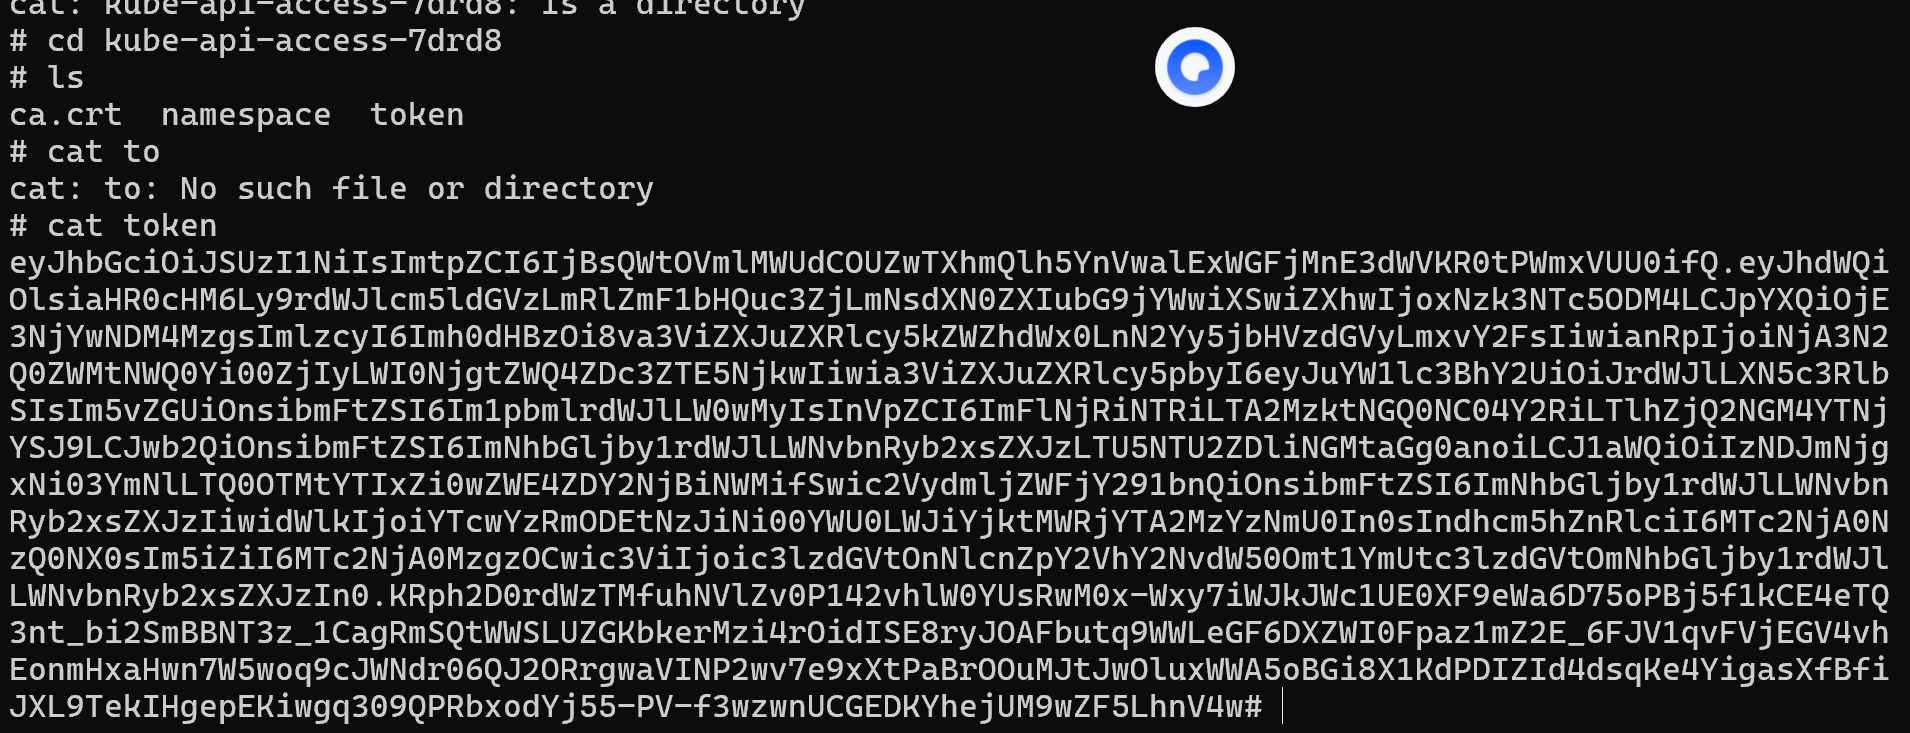
\includegraphics[width=0.95\textwidth]{images/cve3/image.png}
	\caption{CVE-2023-30512：攻击成功证据（基于 CSI ServiceAccount 的越权访问结果）}
	\label{fig:cve-2023-30512-overview}
\end{figure}

\textbf{（2）漏洞复现（验证性复现）}

考虑到本文面向论文复现实验，且该漏洞的攻击细节容易被滥用，本文采用\textbf{验证性复现}思路：
以“RBAC 权限证据 + 受控权限验证”为主，证明 \texttt{cfs-csi-service-account} 具备不应存在的 \texttt{secrets} 读取能力；
同时在策略部署后复测，验证该能力被有效移除。
完整命令与策略清单见附录\ref{app:cve-2023-30512}。

\textbf{环境配置（摘要）}：
\begin{itemize}
	\item Kubernetes 测试集群（Kind/Minikube/实验集群均可，版本以实验环境为准）；
	\item 部署受影响版本的 CubeFS CSI（通过 Helm 或 YAML 部署，命名空间以实际为准）；
	\item 明确 CSI 使用的 ServiceAccount（如 \texttt{cfs-csi-service-account}）以及绑定的 ClusterRole/ClusterRoleBinding。
\end{itemize}

\textbf{复现步骤（摘要）}：
\begin{enumerate}
	\item 盘点并导出 CSI 的 RBAC 绑定，确认 ClusterRole 规则中包含 \texttt{resources:["secrets"]} 且 verbs 包含 \texttt{get/list/watch}；
	\item 以该 ServiceAccount 身份执行权限验证（\texttt{kubectl auth can-i}），确认其具备跨命名空间读取 \texttt{Secret} 的能力；
	\item 按“最小权限 + 准入防回归 + 审计检测”部署策略后，重复第 2 步验证权限应为 \texttt{no}。
\end{enumerate}

\begin{figure}[htbp]
	\centering
	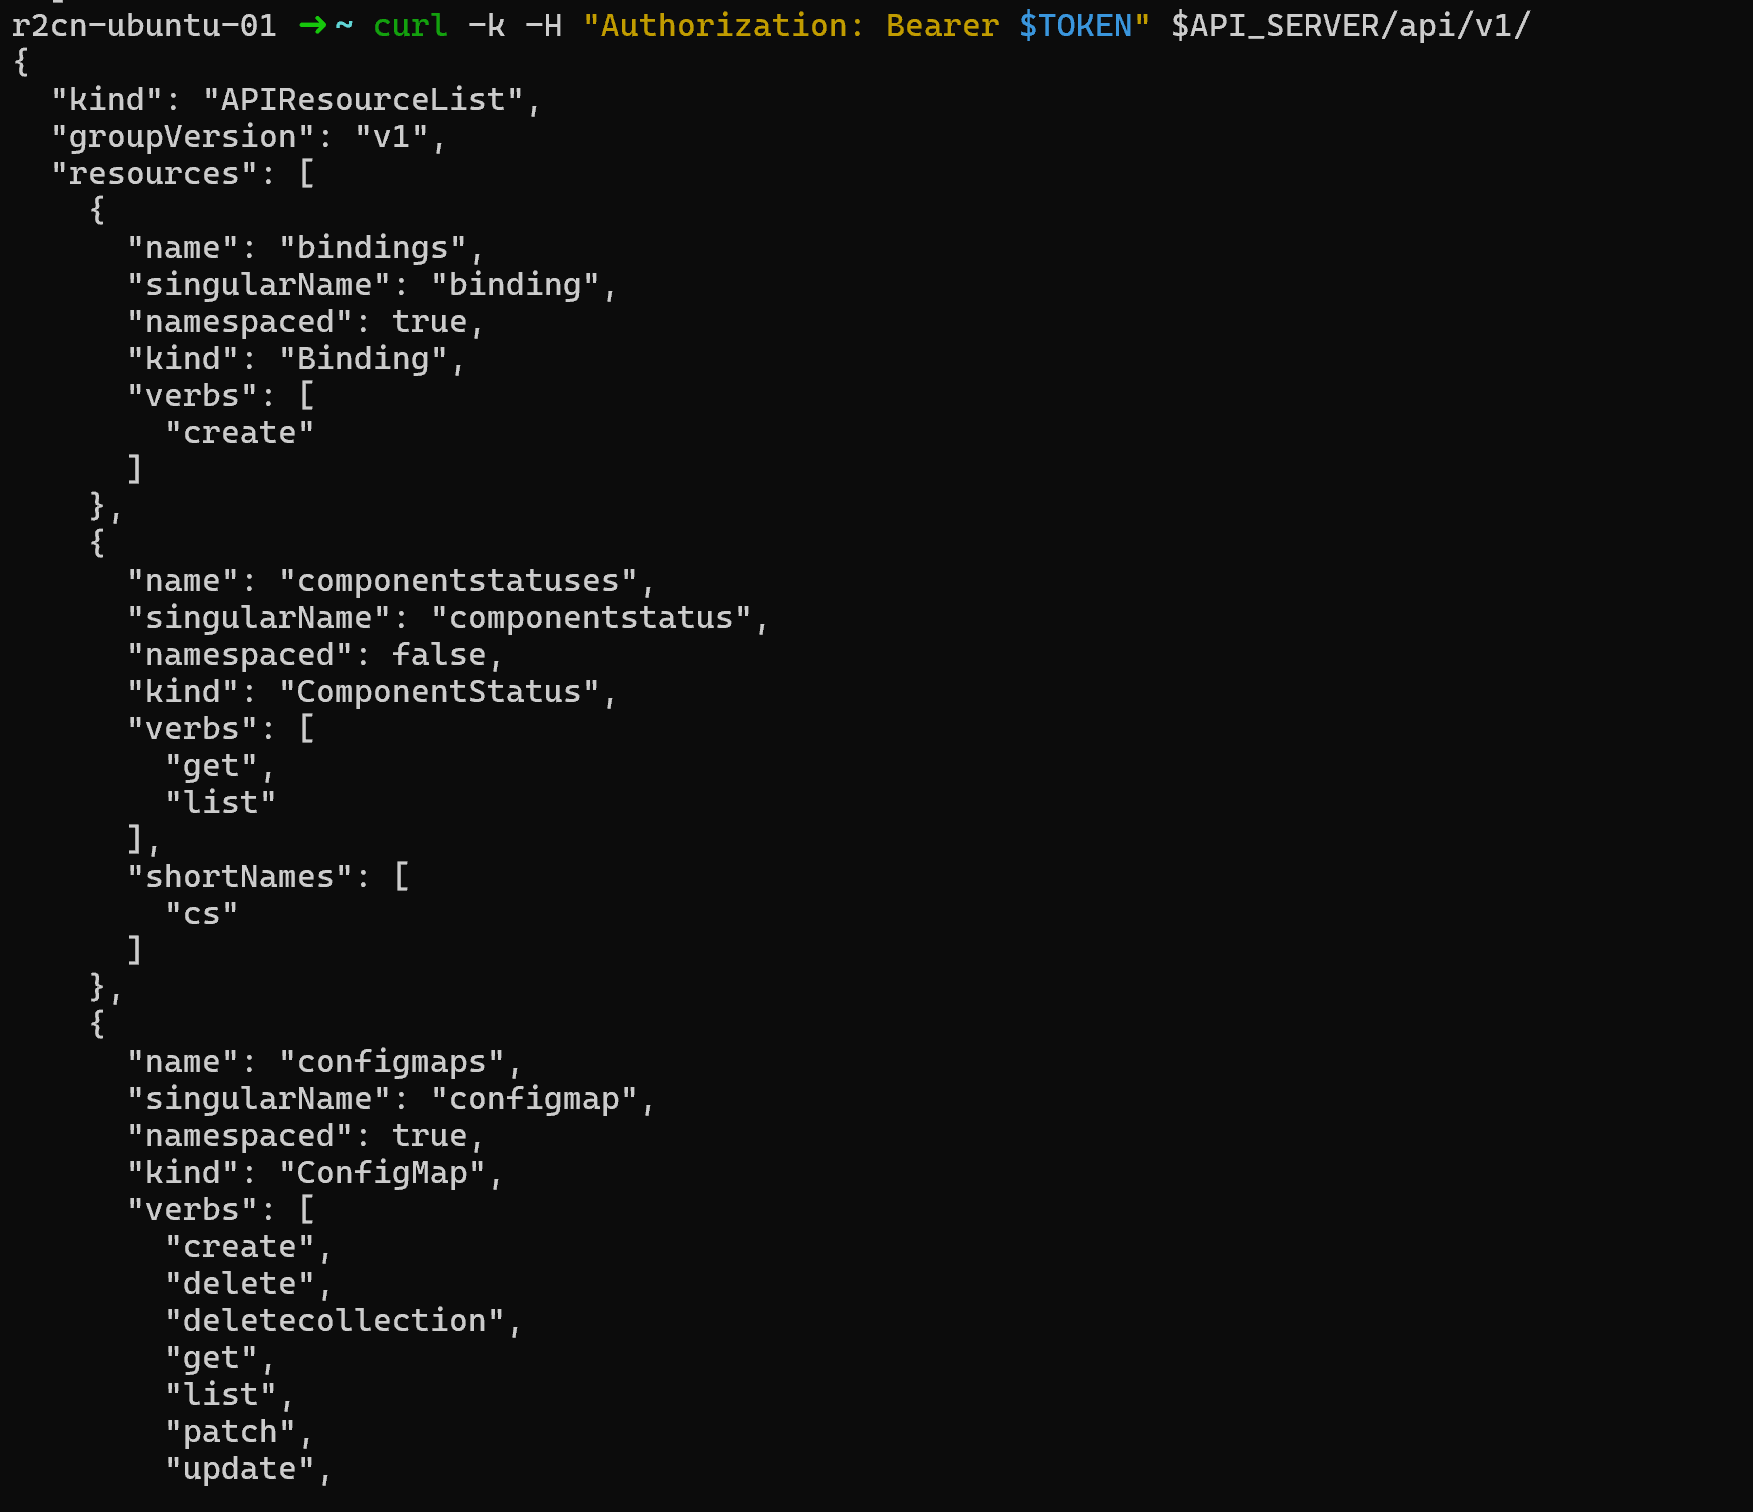
\includegraphics[width=0.95\textwidth]{images/cve3/image2.png}
	\caption{CVE-2023-30512：攻击成功证据（Secrets 读取能力验证/提权结果截图）}
	\label{fig:cve-2023-30512-verify}
\end{figure}

\textbf{攻击结果（摘要）}：若服务账号具备集群范围 \texttt{Secret} 读取权限，则攻击者一旦控制 CSI Pod/节点，存在获取高价值凭据并进一步获得集群控制的风险。


\subsection{策略部署}

本案例的治理重点是\textbf{移除不必要的 Secrets 读取权限}并\textbf{防止权限回归}：
对系统组件而言，升级补丁固然重要，但“RBAC 基线治理 + 准入策略 + 审计检测”能够在补丁不可立即应用或配置漂移场景下提供纵深防护。

\textbf{策略概述}：
\begin{itemize}
	\item \textbf{防控层次（layer）}：身份与权限 / 策略执行 / 审计与检测 / 网络收敛 / 秘密治理
	\item \textbf{防控方法（method）}：RBAC 最小化与清理 + ServiceAccount 硬化（必要时禁用自动挂载令牌） + OPA/Gatekeeper 准入防回归（禁止创建含 \texttt{secrets} 读取动词的 ClusterRole） + 审计检测（对 \texttt{secrets} 枚举告警） + 网络出站收敛（仅允许必要目的地）
	\item \textbf{使用工具}：Kubernetes RBAC、OPA/Gatekeeper（或 Kyverno）、Kubernetes Audit（以及 SIEM/告警系统）、NetworkPolicy
\end{itemize}

\textbf{策略配置与部署步骤}：为避免正文过长，RBAC 最小化示例、准入控制规则、审计策略片段与验证命令见附录\ref{app:cve-2023-30512}。


\subsection{三因素分析}

\textbf{（1）有效性（Effectiveness）}
\begin{itemize}
	\item \textbf{RBAC 最小化}直接移除攻击链关键条件（\texttt{secrets} 读取能力），可从根源降低风险；
	\item \textbf{准入防回归}可阻断后续“误配置/回滚/安装脚本重复引入过度授权”的问题；
	\item \textbf{审计检测}可在异常访问出现时快速发现并触发凭据轮换等止血动作。
\end{itemize}

\textbf{（2）无干扰性（Interference）}
\begin{itemize}
	\item RBAC 收敛可能影响 CSI 的部分诊断/自愈路径，应在预生产环境验证 PVC/PV 生命周期与 attach/detach 流程；
	\item 准入策略若采用 \texttt{deny} 强制模式，需避免误拦截平台必需组件的合法权限；建议先 \texttt{dryrun/audit} 运行并基于白名单迭代；
	\item 审计与检测会增加日志量与告警治理成本，但通常不影响业务链路。
\end{itemize}

\textbf{（3）可部署性（Deployability）}
\begin{itemize}
	\item RBAC 与审计为平台原生能力，可在多集群场景模板化推广；
	\item 准入策略与网络收敛属于“长期基线治理”，可通过 GitOps 与策略即代码持续交付；
	\item 建议提供回滚与灰度路径：先在测试/预生产验证，再逐步推广到生产。
\end{itemize}

